
\setcounter{section}{0}
\section{Trắc nghiệm}
\begin{enumerate}[label=\bfseries Câu \arabic*:]
	
	\item \mkstar{1}
	
	
	{Câu nào sau đây là đúng khi nói về sự rơi?
		\begin{mcq}
			\item Khi không có sức cản vật năng rơi nhanh hơn vật nhẹ.
			\item Ở cùng một nơi, mọi vật rơi tự do có cùng gia tốc.
			\item Khi rơi tự do, vật nào ở độ cao lớn hơn sẽ rơi với gia tốc lớn hơn.
			\item Vận tốc của vật chạm đất không phụ thuộc vào độ cao của vật khi rơi.
		\end{mcq}
	}
	
	\hideall
	{	\textbf{Đáp án: B.}
		
		Gia tốc rơi tự do không phụ thuộc vào khối lượng của vật, chỉ phụ thuộc vào vĩ độ đia lý, độ cao và cấu trúc địa chất nơi đó nên ở cùng một nơi, mọi vật rơi tự do có cùng gia tốc.
	}
	
	\item \mkstar{2}
	
	
	{Người ta thả một vật rơi tự do, sau $\SI{5}{\second}$ vật chạm đất, $g=\SI{9.8}{\meter/\second^2}$. Độ cao thả vật là
		\begin{mcq}(4)
			\item $\SI{122.5}{\meter}$.
			\item $\SI{61.25}{\meter}$.
			\item $\SI{254}{\meter}$.
			\item $\SI{183,75}{\meter}$.
		\end{mcq}
	}
	\hideall
	{	\textbf{Đáp án: A.}	
		
		Độ cao lúc thả vật là:
		$h=s=\dfrac{1}{2}gt^2=\dfrac{1}{2}\cdot\SI{9.8}{\meter/\second^2}\cdot(\SI{5}{\second})^2=\SI{122.5}{\meter}.$
	}
	\item \mkstar{2}
	
	
	{Cùng một lúc tại mái nhà, bi A được thả rơi còn bi B được ném theo phương ngang. Bi A có khối lượng gấp đôi bi B. Bỏ qua sức cản của không khí thì
		\begin{mcq}
			\item bi A chạm đất trước bi B.
			\item bi B chạm đất trước bi A.
			\item cả hai chạm đất cùng lúc.
			\item chưa đủ điều kiện để kết luận bi A hay bi B chạm đất trước.
		\end{mcq}
		
	}
	\hideall
	{	\textbf{Đáp án: C.}
		
		Sự rơi tự do nhanh hay chậm không phụ thuộc vào khối lượng $\left( t=\sqrt{\dfrac{2h}{g}}\right)$.
		
		Do đó hai bi chạm đất cùng lúc.
	}
	
	
	\item \mkstar{2}
	
	
	{Thả hai vật rơi tự do đồng thời từ hai độ cao $h_1$ và $h_2$. Biết rằng thời gian chạm đất của vật thứ nhất bằng 2 lần của vật thứ hai. Tỉ số $\dfrac{h_1}{h_2}$ là
		\begin{mcq}(4)
			\item $\dfrac{h_1}{h_2}=4$.
			\item $\dfrac{h_1}{h_2}=\dfrac{1}{2}$.
			\item $\dfrac{h_1}{h_2}=2$.
			\item $\dfrac{h_1}{h_2}=\dfrac{1}{4}$.
		\end{mcq}
	}
	\hideall
	{	\textbf{Đáp án: A.}
		
		Tỉ số $\dfrac{h_1}{h_2}$ có thể được suy ra từ việc lập tỉ số độ cao của hai vật: $$\dfrac{h_1}{h_2}=\dfrac{\dfrac{1}{2}gt_1^2}{\dfrac{1}{2}gt_2^2}=\dfrac{t_1^2}{t_2^2}=\left( \dfrac{t_1}{t_2}\right)^2=4.$$
	}
	
	\item \mkstar{2}
	
	
	{Một hòn đá thả rơi tự do từ đỉnh toà nhà $25$ tầng nó chạm đất trong thời gian $5\ \text{s}$. Lấy $g=10\ \text{m/s}^2$. Trong giây đầu tiên hòn đá đã đi qua số tầng của toà nhà là
		\begin{mcq}(4)
			\item $1$.
			\item $2$.
			\item $3$.
			\item $5$.
		\end{mcq}
	}
	\hideall
	{	\textbf{Đáp án: A.}
		
		Gọi chiều cao mỗi tầng nhà là $h$. 
		
		Suy ra $25h=g\dfrac{5^2}{2}\Rightarrow h=5\ \text{m}$.
		
		Gọi $n$ là số tầng trong giây đầu hòn đá rơi được.
		
		Suy ra $n\cdot 5=g\cdot \dfrac{1^2}{g}\Rightarrow n=1$.
	}
	\item \mkstar{3}
	
	
	{Từ đỉnh tháp hai vật A và B được thả rơi tự do. Biết B được thả rơi sau A $1\ \text{s}$. Lấy $g=10\ \text{m/s}^2$. Khoảng cách giữa A và B tại thời điểm sau khi B rơi được $2\ \text{s}$ là
		\begin{mcq}(4)
			\item $5\ \text{m}$.
			\item $10\ \text{m}$.
			\item $20\ \text{m}$.
			\item $25\ \text{m}$.
		\end{mcq}
		
	}
	\hideall
	{	\textbf{Đáp án: D.}
		
		Tại thời điểm sau khi B rơi được $2\ \text{s}$, A đã rơi được $3\ \text{s}$
		
		Suy ra, khoảng cách giữa A và B là:
		
		$\Delta h=g\cdot\dfrac{t_1^2}{2}-g\cdot\dfrac{t_2^2}{2}=\dfrac{10}{2}\cdot \left( 3^2-2^2\right)=25\ \text{m}$.
	}
	\item \mkstar{3}
	
	
	{Một người thả vật rơi tự do, vật chạm đất có $v=\SI{36}{\meter/\second}$, $g=\SI{10}{\meter/\second^2}$. Độ cao của vật sau khi thả được $\SI{3}{\second}$ là
		\begin{mcq}(4)
			\item $\SI{64.8}{\meter}$
			\item $\SI{19.8}{\meter}$
			\item $\SI{86.4}{\meter}$
			\item $\SI{45.0}{\meter}$
		\end{mcq}
	}
	\hideall
	{	\textbf{Đáp án: B.}
		
		Độ cao nơi thả vật:
		$$v=\sqrt{2gh}\Rightarrow h = \SI{64.8}{\meter}.$$
		Quãng đường vật rơi $\SI{3}{\second}$ đầu tiên là:
		$$s_3=\dfrac{1}{2}gt^2=\dfrac{1}{2}\cdot\SI{10}{\meter/\second^2}\cdot(\SI{3}{\second})^2=\SI{45}{\meter}.$$
		Độ cao của vật lúc này:
		$$h=s-s_3=\SI{64.8}{\meter}-\SI{45}{\meter}=\SI{19.8}{\meter}.$$
	}
	\item \mkstar{3}
	
	
	{Các giọt nước mưa đang rơi từ mái nhà xuống sau những khoảng thời gian bằng nhau. Khi giọt thứ nhất chạm đất thì giọt thứ năm bắt đầu rơi, lúc đó khoảng cách giữa giọt thứ nhất và giọt thứ hai là $\SI{14}{\meter}$. Lấy $g=\SI{10}{\meter/\second^2}$. Độ cao mái nhà là
		\begin{mcq}(4)
			\item $\SI{32}{\meter}$.
			\item $\SI{9}{\meter}$.
			\item $\SI{56}{\meter}$.
			\item $\SI{16}{\meter}$.
		\end{mcq}
	}
	\hideall
	{	\textbf{Đáp án: A.}
		
		Gọi $\Delta t$ khoảng thời gian bằng nhau các giọt nước mưa đang rơi từ mái nhà xuống.
		
		Quãng đường giọt thứ nhất rơi cho đến khi chạm đất là:
		$$s_1=\dfrac{1}{2}g(4\Delta t)^2.$$
		Quãng đường giọt thứ hai rơi cho đến khi giọt thứ nhất chạm đất là:
		$$s_2=\dfrac{1}{2}g(3\Delta t)^2.$$
		Theo đề bài ta có:
		$$\Delta s= s_1-s_2=\dfrac{7}{2}g(\Delta t)^2=\SI{14}{\meter}\Rightarrow \Delta t=\dfrac{\sqrt{10}}{5}\,\text{s}.$$
		Độ cao mái nhà là:
		$$h=s_1=\dfrac{1}{2}g(4\Delta t)^2=\SI{32}{\meter}.$$
	}
	
	
	\item \mkstar{3}
	
	
	{Một vật rơi tự do từ độ cao $250\ \text{m}$. Tỉ số quãng đường vật rơi được trong $2\ \text{s}$ đầu, $2\ \text{s}$ sau và $2\ \text{s}$ cuối cùng là
		\begin{mcq}(4)
			\item $1:4:9$.
			\item $1:2:4$.
			\item $1:3:5$.
			\item $1:2:3$.
		\end{mcq}
	}
	\hideall
	{	\textbf{Đáp án: C.}
		
		Rơi tự do là chuyển động nhanh dần đều với $V_0=0$  nên khi thời gian chuyển động trên các đoạn đường liên tiếp bằng nhau (cùng bằng $2\ \text{s}$) thì: $\Delta s_1:\Delta s_2:\Delta s_3=1:3:5$.
	}
	\item \mkstar{4}
	
	
	{Quãng đường vật rơi trong giây thứ $n$ là $h$. Quãng đường mà nó rơi trong giây tiếp theo là
		\begin{mcq}(4)
			\item $h$.
			\item $\left(h+\dfrac{g}{2}\right)$.
			\item $(h-g)$.
			\item $(h+g)$.
		\end{mcq}
		
		
	}
	\hideall
	{	\textbf{Đáp án: D.}
		
		Quãng đường vật rơi được trong giây thứ $n$ bằng quãng đường vật rơi được từ ban đầu cho đến giây $n$ trừ cho quãng đường vật rơi được từ ban đầu cho đến giây $n-1$: $$h=\dfrac{1}{2}gn^2-\dfrac{1}{2}g(n-1)^2=\dfrac{g}{2}(2n-1)$$
		
		Quãng đường vật rơi được trong giây thứ $n+1$ bằng quãng đường vật rơi được từ ban đầu cho đến giây $n+1$ trừ cho quãng đường vật rơi được từ ban đầu cho đến giây $n$:
		$$h'=\dfrac{1}{2}g(n+1)^2-\dfrac{1}{2}gn^2 = \dfrac{g}{2}(2n+1)$$
		
		Vậy $h'=h+g$.
	}
\end{enumerate}


\hideall
{
	\begin{center}
		\textbf{BẢNG ĐÁP ÁN}
	\end{center}
	\begin{center}
		\begin{tabular}{|m{2.8em}|m{2.8em}|m{2.8em}|m{2.8em}|m{2.8em}|m{2.8em}|m{2.8em}|m{2.8em}|m{2.8em}|m{2.8em}|}
			\hline
			1.B  & 2.A  & 3.C  & 4.A  & 5.A  & 6.D  & 7.B  & 8.A  & 9.C  & 10.D  \\
			\hline
			
		\end{tabular}
	\end{center}
}
\section{Tự luận}
\begin{enumerate}[label=\bfseries Câu \arabic*:]
	\item \mkstar{1}
	
	{
		Sự rơi tự do là gì? Nêu các đặc điểm của sự rơi tự do.
	}
	
	\hideall{
		
		Sự rơi tự do là sự rơi của các vật chỉ dưới tác dụng của trọng lực.
		
		Các đặc điểm của sự rơi tự do:
		\begin{itemize}
			\item Phương của chuyển động rơi tự do là phương thẳng đứng;
			\item Chiều của chuyển động rơi tự do là chiều từ trên xuống dưới;
			\item Chuyển động rơi tự do là chuyển động thẳng nhanh dần đều.
		\end{itemize}
	}
		\item \mkstar{2}
	
	{
		Một vật được thả rơi không vận tốc đầu khi vừa chạm đất có $v=\SI{70}{m/s}$, $g = \SI{10}{m/s}^2$.
		\begin{enumerate}[label=\alph*)]
			\item Xác định quãng đường rơi của vật.
			\item Tính thời gian rơi của vật.
		\end{enumerate}
	}
	
	\hideall{
		
		\begin{enumerate}[label=\alph*)]
			\item Quãng đường rơi của vật
			
			$$v^2 - v^2_0 = 2gS \Rightarrow S = \dfrac{v^2-v^2_0}{2a} = \SI{245}{m}.$$
			
			\item Thời gian rơi của vật
			
			$$v = gt \Rightarrow t = \dfrac{v}{g} =\SI{7}{s}.$$
		\end{enumerate}

	}
		\item \mkstar{2}
		{
			
	Từ độ cao $\SI{120}{m}$ người ta thả một vật thẳng đứng xuống với $v = \SI{10}{m/s}, g = \SI{10}{m/s}^2$.
	\begin{enumerate}[label=\alph*)]
		\item Sau bao lâu vật chạm đất?
		\item Tính vận tốc của vật lúc vừa chạm đất.
	\end{enumerate}
	}
	
	\hideall{
		
		\begin{enumerate}[label=\alph*)]
			\item Thời gian vật chạm đất
			
			$$s = v_0t + \dfrac{1}{2}gt^2 \Rightarrow t =\SI{4}{s}.$$
			
			\item Vận tốc của vật lúc vừa chạm đất
			
			$$v = v_0 +gt = \SI{50}{m/s}.$$
		\end{enumerate}
	}
		\item \mkstar{2}
		{
			
		Thả một hòn đá từ độ cao $h$ xuống đấy, hòn đá rơi trong $\SI{1}{s}$. Nếu thả hòn đá đó từ $h’ = 4h$ thì thời gian rơi là bao nhiêu?
	}
	
	\hideall{
		
		Ta có:
		
		$$h = \dfrac{1}{2} gt^2 \Rightarrow t =\sqrt{\dfrac{2h}{g}} = \SI{1}{s}.$$
		
		Lại có:
		
		$$h' = \dfrac{1}{2}gt_1^2 \Rightarrow t_1 = \sqrt{\dfrac{2h'}{g}} =\SI{2}{s}.$$
		
	}
	\item \mkstar{2}
	
	{Một vật nặng rơi từ độ cao 20 m xuống đất. Tính thời gian rơi và vận tốc của vật khi chạm đất. Lấy $g=\SI{10}{m/s^2}$.}
	\hideall{
		
		Chọn gốc tọa độ tại điểm rơi, gốc thời gian lúc vật bắt đầu rơi, trục tọa độ có chiều dương hướng thẳng đứng xuống dưới.
		
		Khi vật chạm đất thì:
		$$s=h=\dfrac{gt^2}{2} \Rightarrow t=\sqrt{\dfrac{2h}{g}} = 2\ \text s$$
		
		Vận tốc của vật khi chạm đất:
		$$v=gt = 20\ \text{m/s}$$
	}
	\item \mkstar{3}
	
	
	{
		Một hòn đá rơi tự do từ cửa sổ một toà nhà cao tầng. Sau đó $1\ \text{s}$ tại ban công phía dưới cách cửa sổ trên của toà nhà $20\ \text{m}$ có một hòn đá khác cũng rơi tự do. Biết cả hai hòn đá cùng chạm đất đồng thời. Lấy $g=10\ \text{m/s}^2$. Tìm chiều cao của cửa sổ toà nhà trên so với đất.	
	}
	\hideall
	{	
		
		Ta có: $h=g\cdot \dfrac{t^2}{2}; \ h-20=g\cdot \dfrac{\left(t-1 \right)^2 }{2}$.
		
		$\Rightarrow t=\text{2,5}\ \text{s}; \ h=\text{31,25}\ \text{m}$.  
	}
	\item \mkstar{4}
	
	
	{
		Hai viên bi sắt được thả rơi cùng độ cao cách nhau một khoảng thời gian $\SI{0,5}{\second}$. Lấy $g = \SI{10}{\meter/\second^2}$. Tìm khoảng cách giữa hai viên bi sau khi viên thứ nhất rơi được $\SI{1,5}{\second}$.
	}
	\hideall
	{	
		Chọn gốc thời gian là lúc thả viên bi 1. Viên bi 2 được thả sau $\SI{0,5}{\second}$ nên:
		$$t_2=t_1-\SI{0,5}{\second}$$
		Quãng đường viên bi 1 đi được:
		$$s_1=\frac{1}{2}gt_1^2.$$
		Quãng đường viên bi 2 đi được:
		$$s_2=\frac{1}{2}g(t_1-0,5)^2$$
		Lấy $s_1-s_2=\frac{1}{2}gt_1^2-\frac{1}{2}g(t_1-0,5)^2=\SI{6,25}{\meter}$.
	}
	\item \mkstar{4}
	
	
	{
		Một viên bi A được thả rơi từ độ cao $\SI{30}{\meter}$. Cùng lúc đó, một viên bi B được bắn theo phương thẳng đứng từ dưới đất lên với $\SI{25}{\meter/\second}$ tới va chạm vào bi A. Chọn trục O$y$ thẳng đứng, gốc O ở mặt đất, chiều dương hướng lên, gốc thời gian lúc 2 viên bi bắt đầu chuyển động, $g=\SI{10}{\meter/\second^2}$. Bỏ qua sức cản không khí. Tìm thời điểm và tọa độ 2 viên bi gặp nhau.
	}
	\hideall
	{	
		
		Phương trình chuyển động của viên bi A là:
		$$y_{\text{A}}=y_{0\text{A}}+v_{0\text{A}}t+\dfrac{1}{2}gt^2=30-5t^2 \textrm{ (m, s)}.$$
		Phương trình chuyển động của viên bi B là:
		$$y_{\text{B}}=y_{0\text{B}}+v_{0\text{B}}t+\dfrac{1}{2}gt^2=25t-5t^2\textrm{ (m, s)}.$$
		Hai viên bi gặp nhau khi chúng có cùng tọa độ:
		$$y_{\text{A}}=y_{\text{B}}\Rightarrow 30-5t^2=25t-5t^2 \Rightarrow t=\SI{1.2}{\second}.$$
		Tọa độ hai viên bi khi gặp nhau là:
		$$y_{\text{A}}=y_{\text{B}}=30-5t^2=\SI{22.8}{\meter}.$$
	}
		\item \mkstar{4}
	
	
	{
		Một người thả một hòn bi từ trên cao xuống đất và đo được thời gian rơi là $\SI{3,1}{s}$. Bỏ qua sức cản không khí. Lấy $g=\SI{9,8}{m/s}^2$.
		\begin{enumerate}[label=\alph*)]
			\item Tính độ cao của nơi thả hòn bi so với mặt đất và vận tốc lúc chạm đất.
			\item Tính quãng đường rơi được trong $\SI{0,5}{s}$ cuối trước khi chạm đất.
		\end{enumerate}
	}
	\hideall
	{	
		\begin{enumerate}[label=\alph*)]
			\item Độ cao của nơi thả hòn bi so với mặt đất 
			
			$$h = \dfrac{1}{2}gt^2 = \SI{47,089}{m}.$$
			
			Vận tốc lúc chạm đất
			
			$$ v = gt = \SI{30,38}{m/s}.$$
			
			\item Quãng đường rơi được trong $\SI{0,5}{s}$ cuối trước khi chạm đất
			
			$$h' = \dfrac{1}{2} g(t - \text{0,5})^2 = \SI{33,124}{m}.$$
		\end{enumerate}
	}
		\item \mkstar{4}
	
	
	{
		Căn cứ vào số liệu cho trong bảng để :
		\begin{center}
			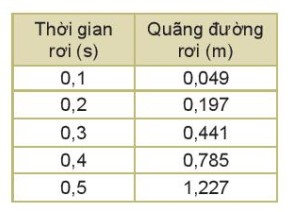
\includegraphics[scale=1]{../figs/VN10-2022-PH-TP013-1.jpg}
		\end{center}
		\begin{enumerate}[label=\alph*)]
			\item Chứng tỏ chuyển động rơi tự do là nhanh dần đều. 
			\item Tính gia tốc của chuyển động rơi tự do.
		\end{enumerate}
	}
	\hideall
	{	
		\begin{enumerate}[label=\alph*)]
			\item 
			+ Từ giây thứ 0,1 đến 0,2, vật rơi được
			
			 $$\Delta S_1 = S_2 -  S_1=\text{0,197} - \text{0,049} = \SI{0,148}{m}$$.
			
			+ Từ giây thứ 0,2 đến 0,3, vật rơi được một khoảng là: 
			
			$$\Delta S_2 = S_3 -  S_2= \text{0,441} - \text{0,197}= \SI{0,244}{m}.$$
			
			+ Từ giây thứ 0,3 đến 0,4, vật rơi được một khoảng là :
			 
			$$\Delta S_3= S_4 - S_3= \text{0,785} - \text{0,441}= \SI{0,344}{m}.$$
			
			Như vậy, sau cùng 1 khoảng là 0,1 giây như nhau nhưng vật rơi được những khoảng khác nhau, càng về sau thì rơi càng nhanh hơn. 
			
			\item Dựa vào công thức:
			
			$$S = \dfrac{1}{2}gt^2 \Rightarrow g = \dfrac{2S}{t^2}.$$
			
			Ta có
			
			+ Gia tốc tại $t_1$  0,1 giây là: 
			
			$$g_1 = \dfrac{2 S_1}{t_1^2}= \SI{9,8}{m/s}^2.$$
				
			+ Gia tốc tại $t_2$ 0,2 giây là: 
			
			$$g_2 = \dfrac{2 S_2}{t_2^2}\SI{9,85}{m/s}^2.$$
					
			+ Gia tốc tại $t_3$ 0,3 giây là: 
			
			$$g_3 = \dfrac{2 S_3}{t_3^2}=\SI{9,8}{m/s}^2.$$
			
			+ Gia tốc tại $t_4$ 0,4 giây là: 
			$$g_4 = \dfrac{2S_4}{t_4^2}=\SI{9,8125}{m/s}^2.$$
			
			
		\end{enumerate}
	}
\end{enumerate}